\documentclass[11pt,aspectratio=169,dvipsnames]{beamer}
\graphicspath{{figs/}}
\usetheme{default}
\usepackage{DasBeamerPaket}
\usepackage{animate}
\usepackage{lastpage}
\usepackage{enumitem}
\usepackage{appendixnumberbeamer}
\usepackage{braket}
\usepackage{tikz}
\setbeamercolor{section in toc}{fg=NavyBlue}
\setbeamercolor{frametitle}{fg=NavyBlue}
\captionsetup[figure]{labelfont=bf}
\captionsetup[table]{labelfont=bf}
\newcommand{\theauthor}{Jakob Krause}
\newcommand{\theshortauthor}{\textsc{J. Krause} for CBELSA/TAPS}
\newcommand{\authormail}{krause@hiskp.uni-bonn.de}
\newcommand{\authorgit}{krausejm}
\newcommand{\thetitle}{Recent Polarization Observable Results in  $\eta$- and $\eta'$-photoproduction off the proton}
\newcommand{\theshorttitle}{$\Sigma$ in $\eta$- and $\eta'$ photoproduction}
\newcommand{\thecolor}{black!70!blue}
\newcommand{\thecolorr}{black!60!blue}
\newcommand{\thecolorrr}{black!50!blue}
\newcommand{\thesubtitle}{Master thesis for the CBELSA/TAPS collaboration}
\newcommand{\thedate}{30th March 2022}
\makeatletter
\patchcmd{\beamer@calculateheadfoot}{\advance\footheight by 4pt}{\advance\footheight by 20pt}{}{}
\makeatother
\begin{document}
	\definecolor{myWhite}{rgb}{1,1,1}
	
	
	\setbeamercolor{coloredboxstuff}{fg=myWhite,bg=\thecolor}
	\setbeamercolor{coloredboxstuff1}{fg=myWhite,bg=\thecolorr}
	\setbeamercolor{coloredboxstuff2}{fg=myWhite,bg=\thecolorrr}	
	\makeatother
	\setbeamertemplate{footline}
	{
		\leavevmode%
		\hbox{%
			\begin{beamercolorbox}[wd=.33\paperwidth,ht=2.25ex,dp=1ex,center]{coloredboxstuff}%
				{\theshortauthor}
			\end{beamercolorbox}%
			\begin{beamercolorbox}[wd=.34\paperwidth,ht=2.25ex,dp=1ex,center]{coloredboxstuff1}%
				{\theshorttitle}
			\end{beamercolorbox}%
			\begin{beamercolorbox}[wd=.33\paperwidth,ht=2.25ex,dp=1ex,center]{coloredboxstuff}%
				\insertframenumber{} / \inserttotalframenumber\hspace*{1ex}
		\end{beamercolorbox}}%
	}
	\makeatletter
	
	
	\setbeamercovered{transparent}
	\setbeamertemplate{navigation symbols}{}
	\setbeamertemplate{frametitle}[default][left,leftskip=0.5cm]
	\setbeamertemplate{itemize item}{\color{black}$\blacktriangleright$}
	\setbeamertemplate{section in toc}[sections numbered]
	\setbeamercolor{section in toc}{fg=\thecolor}
	\setbeamercolor{frametitle}{fg=\thecolor}
	\captionsetup{font=scriptsize,labelfont=scriptsize}
	\AtBeginSection[]
	{	
		
		{
			
			\makeatother
			\setbeamertemplate{footline}
			{
				\leavevmode%
				\hbox{%
					\begin{beamercolorbox}[wd=.34\paperwidth,ht=2.25ex,dp=1ex,center]{coloredboxstuff}%
						{|\hfill\theshortauthor\hfill|}
					\end{beamercolorbox}%
					\begin{beamercolorbox}[wd=.34\paperwidth,ht=2.25ex,dp=1ex,center]{coloredboxstuff}%
						{\theshorttitle}
					\end{beamercolorbox}%
					\begin{beamercolorbox}[wd=.34\paperwidth,ht=2.25ex,dp=1ex,center]{coloredboxstuff}%
						\insertsection\hspace*{1ex}
				\end{beamercolorbox}}%
			}
			\makeatletter
			
			
			\begin{frame}[noframenumbering]
				\frametitle{}
				\addtocounter{page}{-1}
				\tableofcontents[currentsection]
			\end{frame}
		}
		
	}
	%\begin{frame}[plain]
	%	\centering
	%	{\Large \color{\thecolor}{\thetitle}}\\
	%	\vspace{0.5cm}
	%	{\thesubtitle}
	%	\vfill
	%	\begin{minipage}{\linewidth}
		%		\centering
		%		\begin{minipage}{\linewidth}
			%			\textsc{\theauthor}\\
			%			\scriptsize \href{mailto:\authormail}{\faEnvelope  \hspace*{0.1cm}\authormail} {\color{black}$|$} \href{https://github.com/\authorgit}{\faGithub  \hspace*{0.1cm}\authorgit}\\
			%		\end{minipage}
		%		\vspace{.5cm}
		
		%		{\scriptsize
			%			Supervisor: \textsc{Jun. Prof. Dr. Annika Thiel}\\
			%			\tiny \href{mailto:thiel@hiskp.uni-bonn.de}{\faEnvelope  \hspace*{0.1cm}thiel@hiskp.uni-bonn.de}\par}
		%	\end{minipage}
	%	\vspace{0.2cm}
	
	%	\thedate
	%\end{frame}
	
	\begin{frame}{Extracting the beam asymmetry $\Sigma$ from data (bins in ($E_\gamma$,$\cos\theta$))}
		
			\textbf{Event yield asymmetries (binned in $\boldsymbol{\phi}$)}
			$$A(\phi)=\frac{N^\bot-N^\parallel}{p_{\gamma}^\parallel N^\bot+p_{\gamma}^\bot N^\parallel}=\Sigma\cos(2(\alpha^\parallel-\phi))$$


			\textbf{Event based fit (unbinned in $\boldsymbol{\phi}$)}
			\begin{align*}
				-\ln\mathcal{L}=&\sum_{i=1}^{n}-\ln(p_\text{prompt}(\phi_i,p_{\gamma,i},\Sigma,a_1\dots a_4,b_1\dots b_4))+\\
				&\sum_{j=1}^{m}-\ln\left(p_\text{sideband}(\phi_j,p_{\gamma,j},\Sigma^\text{bkg},a_1^\text{bkg}\dots a_4^\text{bkg},b_1^\text{bkg}\dots b_4^\text{bkg})\right)
			\end{align*}
		toy MC: generate events that follow pdfs ($\frac{\text{d}\sigma}{\text{d}\Omega}$) of $N^\parallel,N^\bot$ and $p_\text{prompt},p_\text{sideband}$
	\end{frame}
	\begin{frame}{Investigating toy MC fit results}

	\textbf{$\chi^2$ fits}: investigate \emph{normalized residuals} $\xi=\frac{\Sigma_\text{estimated}-\Sigma_\text{true}}{\text{err}(\Sigma_\text{estimated})}$, \\
	$\to$ "good" fit yields $\xi\sim\mathcal{N}(0,1)$\\
	\textbf{\text{bayesian} fits:} 
	\begin{enumerate}[label=\alph*.]
		\item add up posteriors $p(\Sigma|y_i)$ to combined posterior $P(\Sigma|y_0,\dots,y_{9999})$ (mixture model)\\
		$\to$ expect $P(\Sigma|y_0,\dots,y_{9999})\sim\mathcal{N}(\Sigma_\text{true},\sigma)$
		\item build "normalized residuals" $\Xi=\sum_{i=0}\frac{p(\Sigma|y_i)-\Sigma_\text{true}}{\text{std}(p(\Sigma|y_i))}$\\
		$\to$ expect $\Xi\sim\mathcal{N}(0,\mathcal{O}(1))$
	\end{enumerate} 
also check $\chi^2$ distribution and MCMC diagnostics

		
	\end{frame}
	\begin{frame}{Fit results (event yield asymmetries with \textsc{Bayes})}
		statistics of $\eta$ final state: (12 bins in $\phi$)
		\begin{itemize}[label=$\blacktriangleright$]
			\item 10000 toy bins
			\item $p_\gamma^\parallel=0.25,p_\gamma^\bot=0.3$, $\Sigma=0.3$
			\item $n_\text{events}^\parallel\sim\text{Pois}(800)$, $n_\text{events}^\bot\sim\text{Pois}(1000)$ 
		\end{itemize}
	\begin{figure}[htbp]
		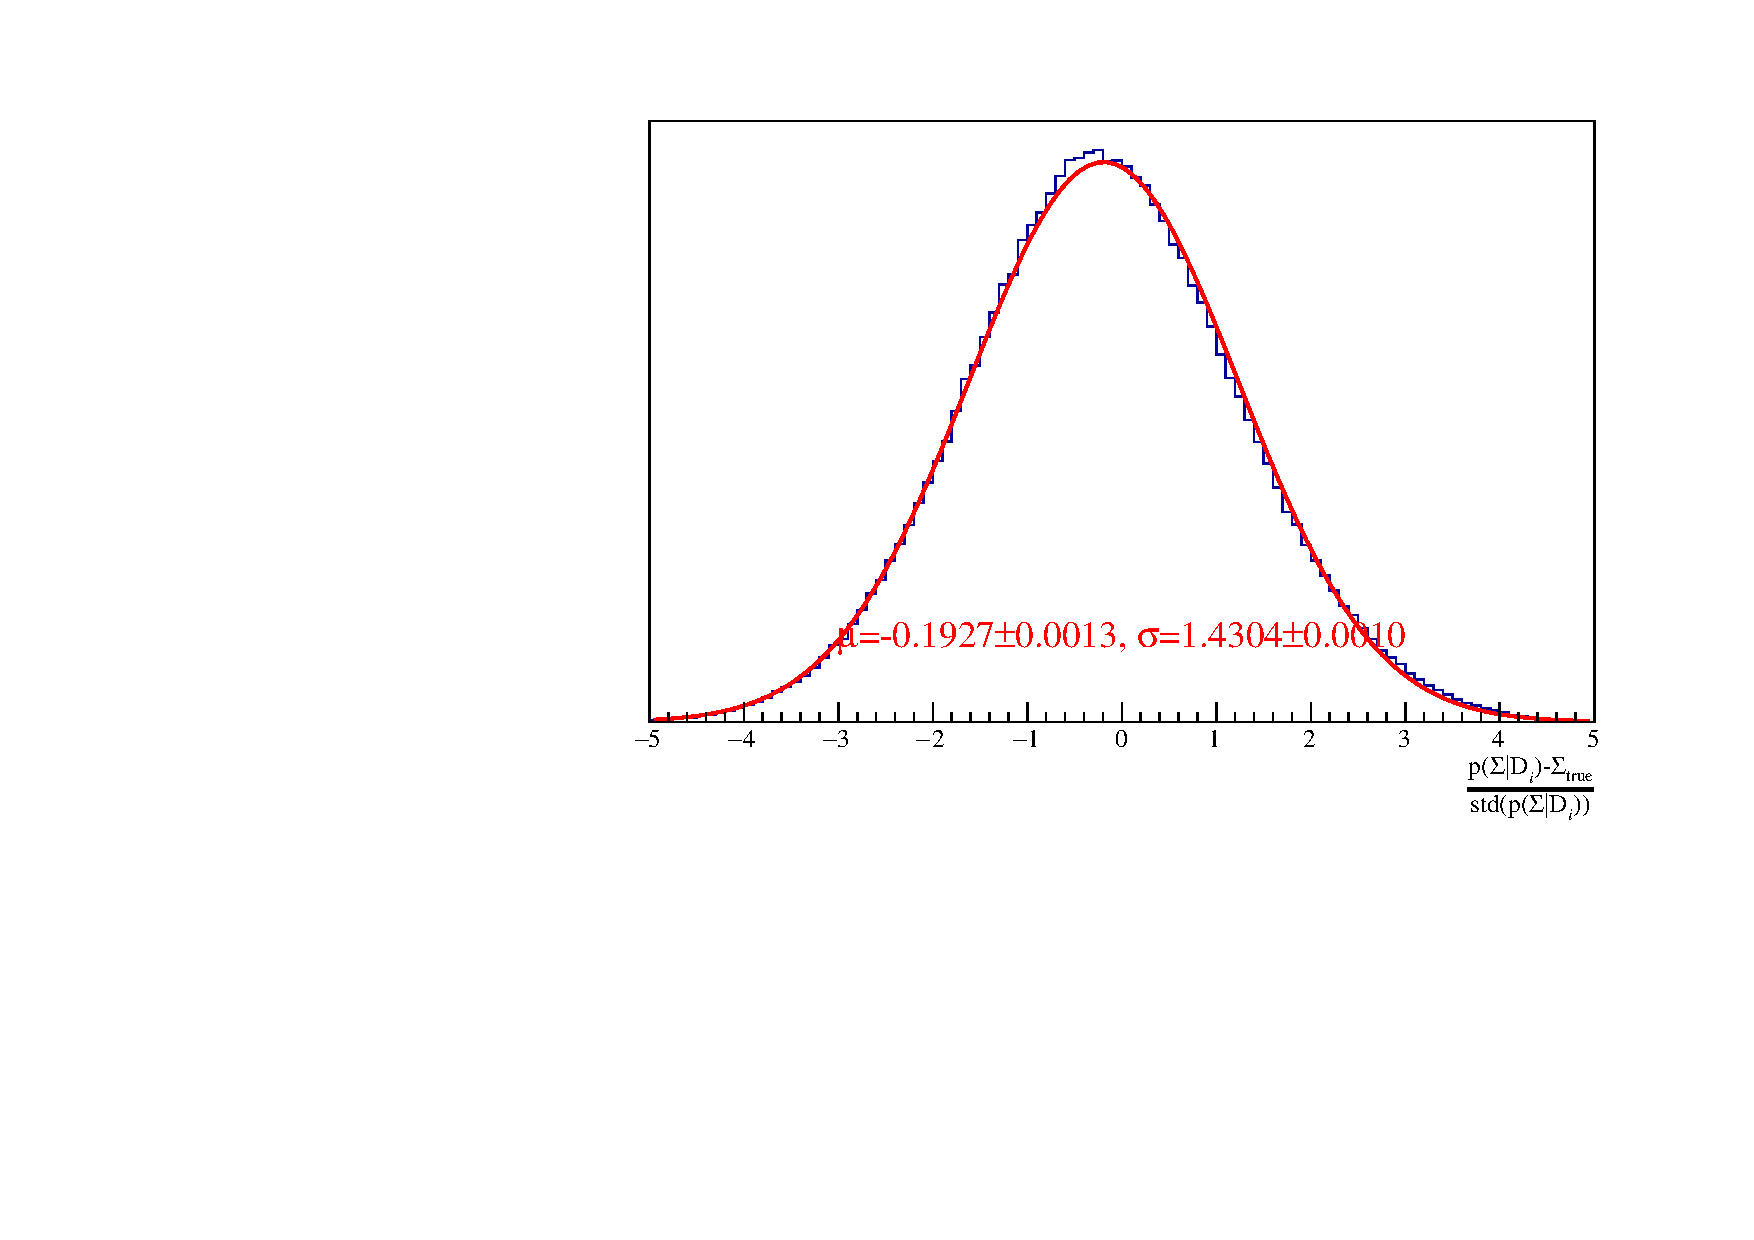
\includegraphics[width=.49\linewidth]{../../bayes/toyMC/plots/combined_post_add.pdf}
		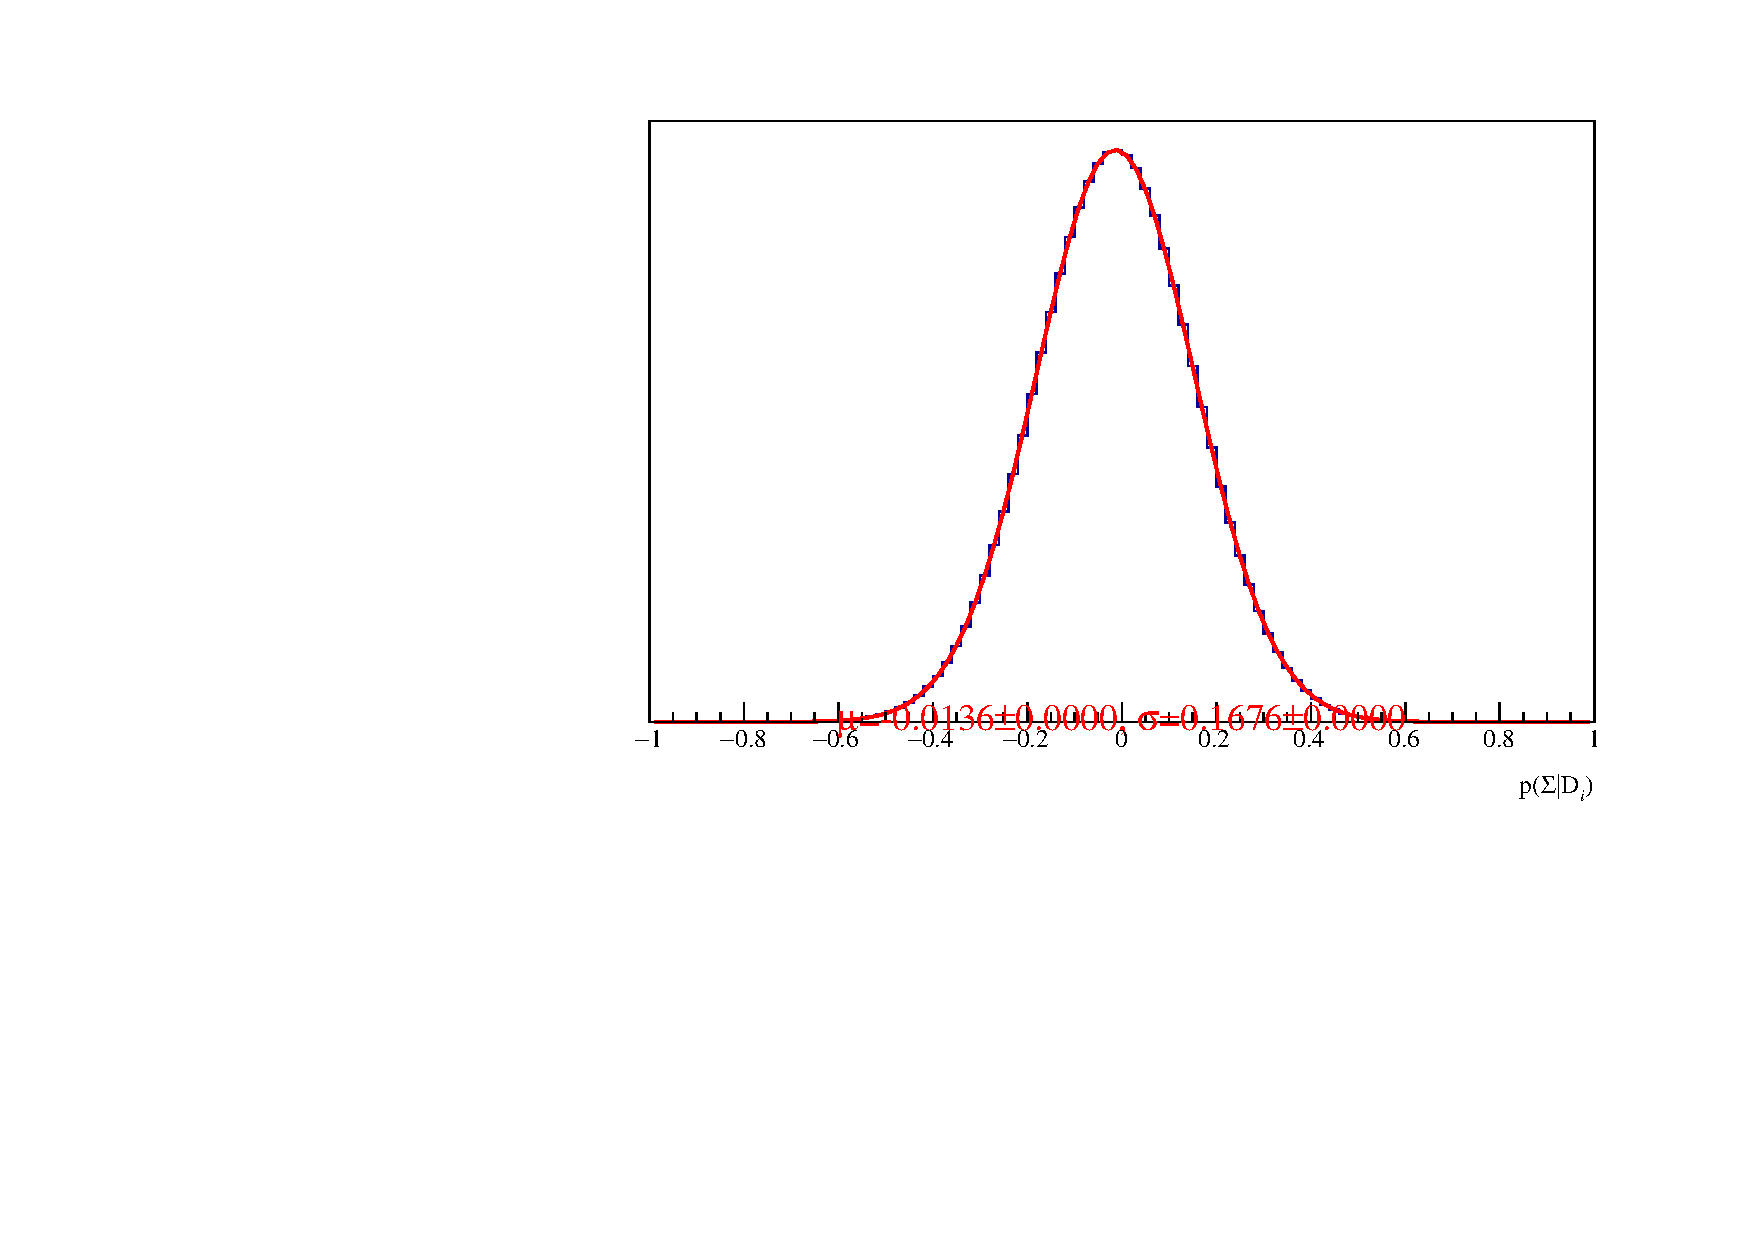
\includegraphics[width=.49\linewidth]{../../bayes/toyMC/plots/combined_post_add_raw.pdf}
	\end{figure}

	\end{frame}
	\begin{frame}{Fit results (event yield asymmetries with $\chi^2$ fit)}
		\begin{center}
		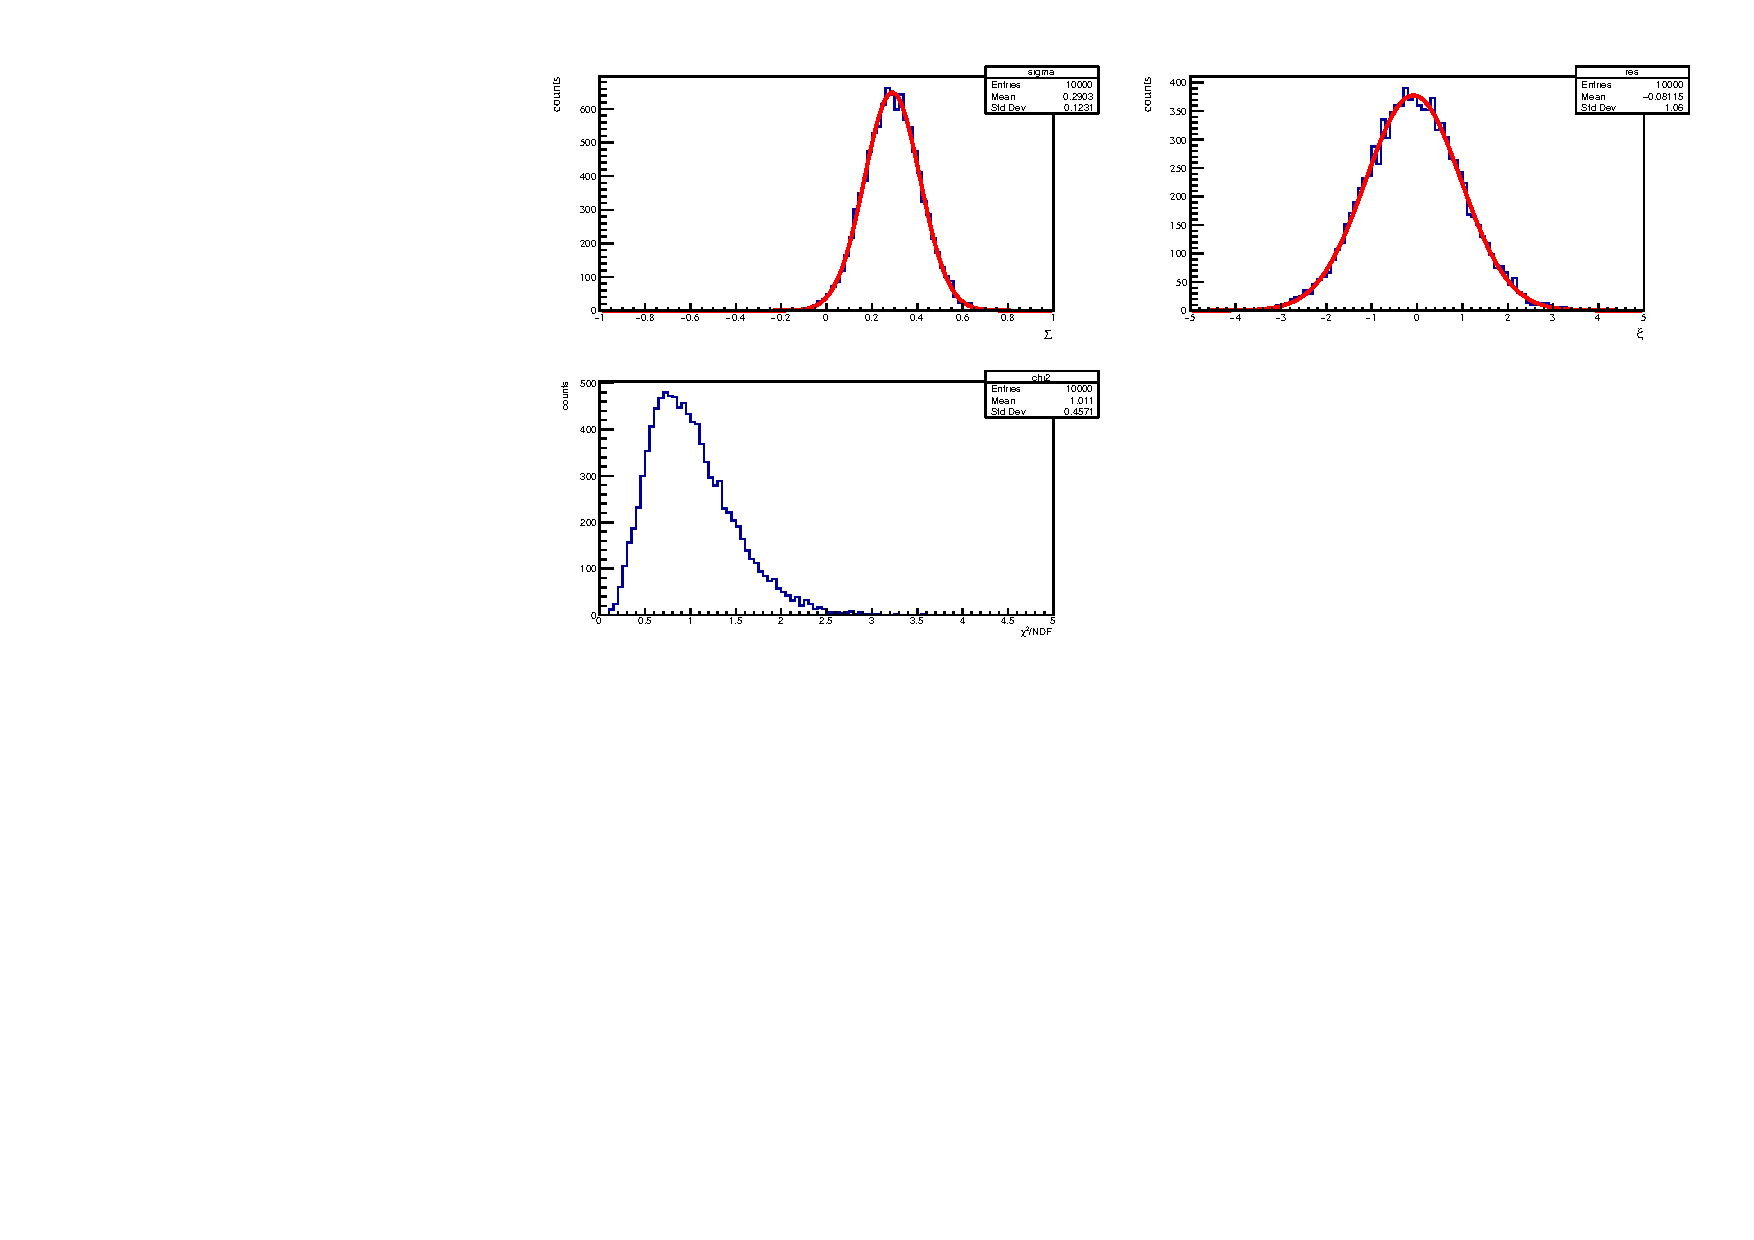
\includegraphics[width=.9\linewidth]{../../bayes/toyMC/plots/eta_chi2_12bins.pdf}
		\end{center}

\end{frame}
		\begin{frame}{Fit results (event yield asymmetries with \textsc{Bayes})}
		statistics of $\pi^0$ final state: (24 bins in $\phi$)
		\begin{itemize}[label=$\blacktriangleright$]
			\item 10000 toy bins
			\item $p_\gamma^\parallel=0.25,p_\gamma^\bot=0.3$, $\Sigma=0.3$
			\item $n_\text{events}^\parallel\sim\text{Pois}(4000)$, $n_\text{events}^\bot\sim\text{Pois}(5000)$ 
		\end{itemize}
		\begin{figure}[htbp]
			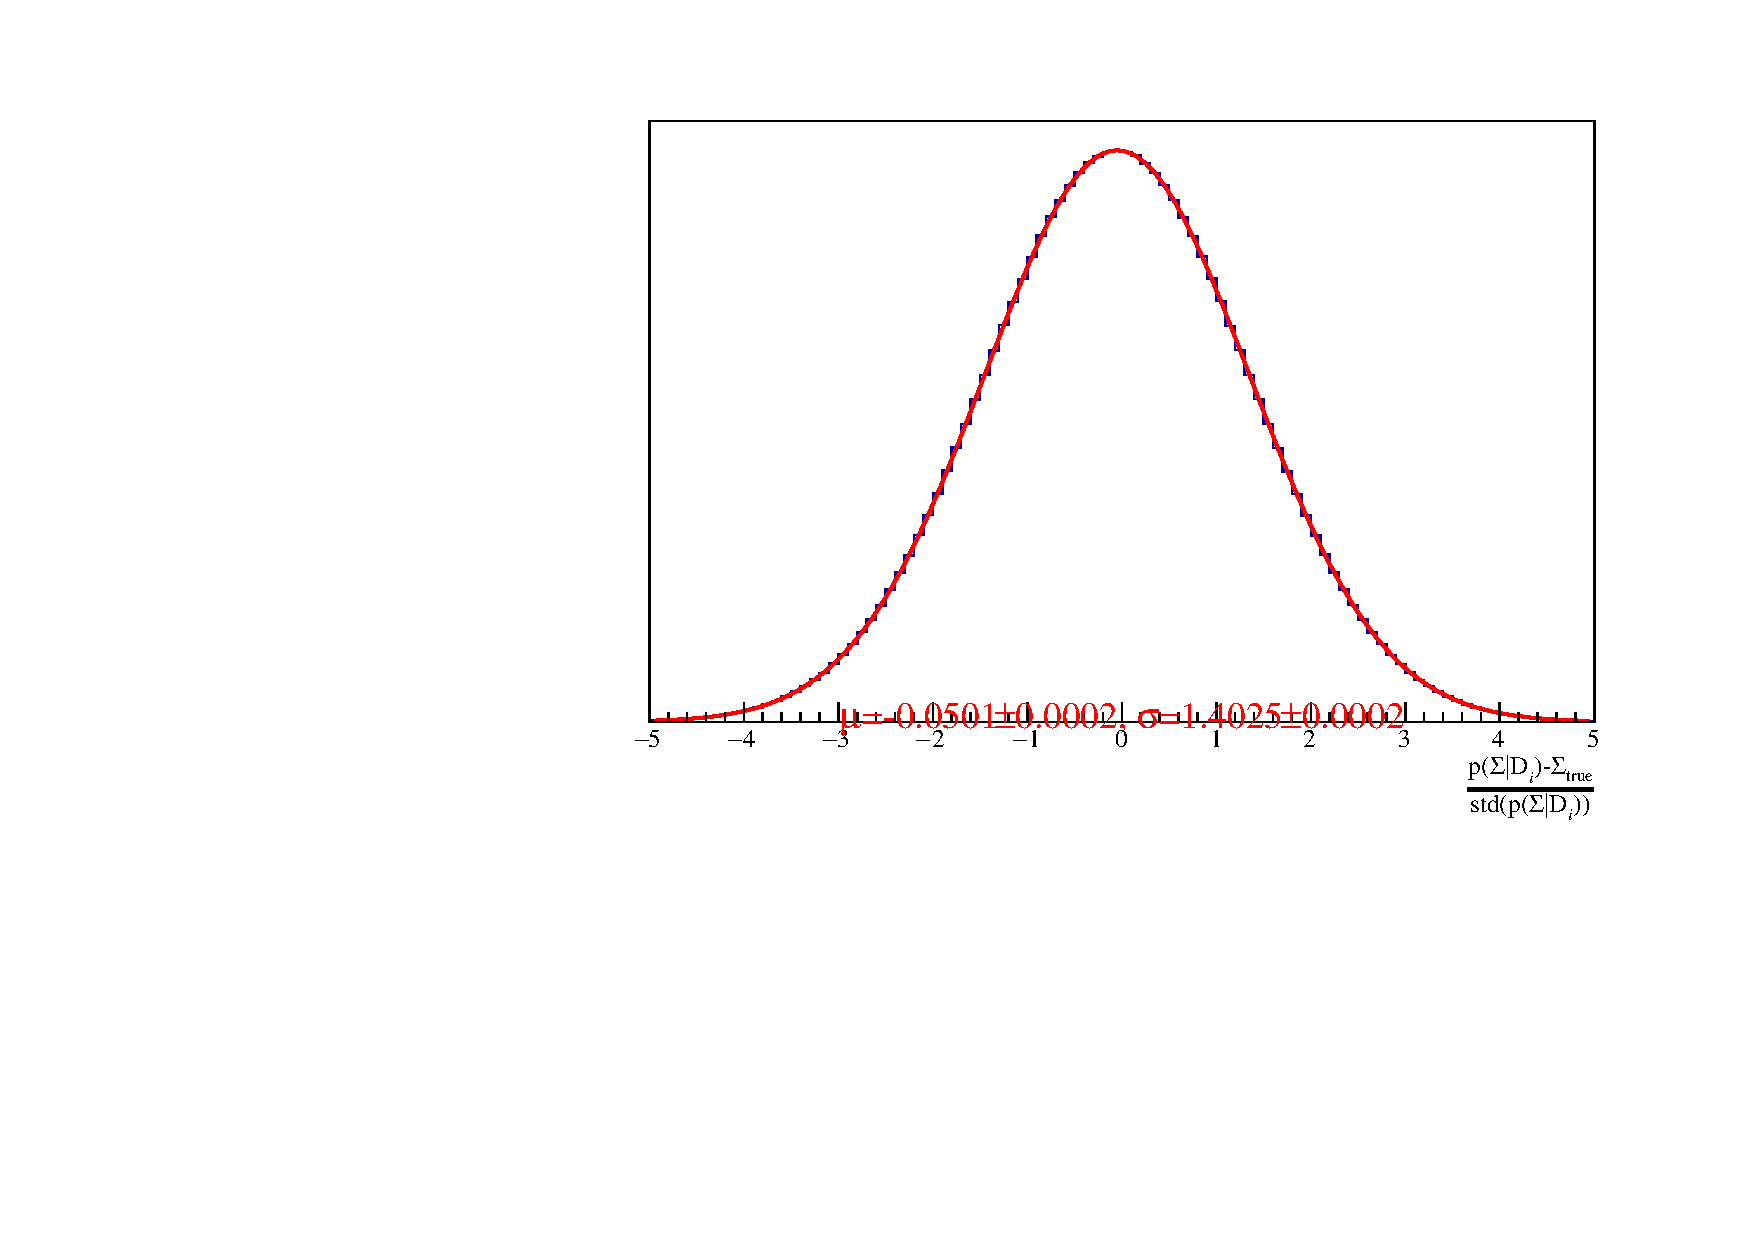
\includegraphics[width=.49\linewidth]{../../bayes/toyMC/plots/pi0_combined_post_add.pdf}
			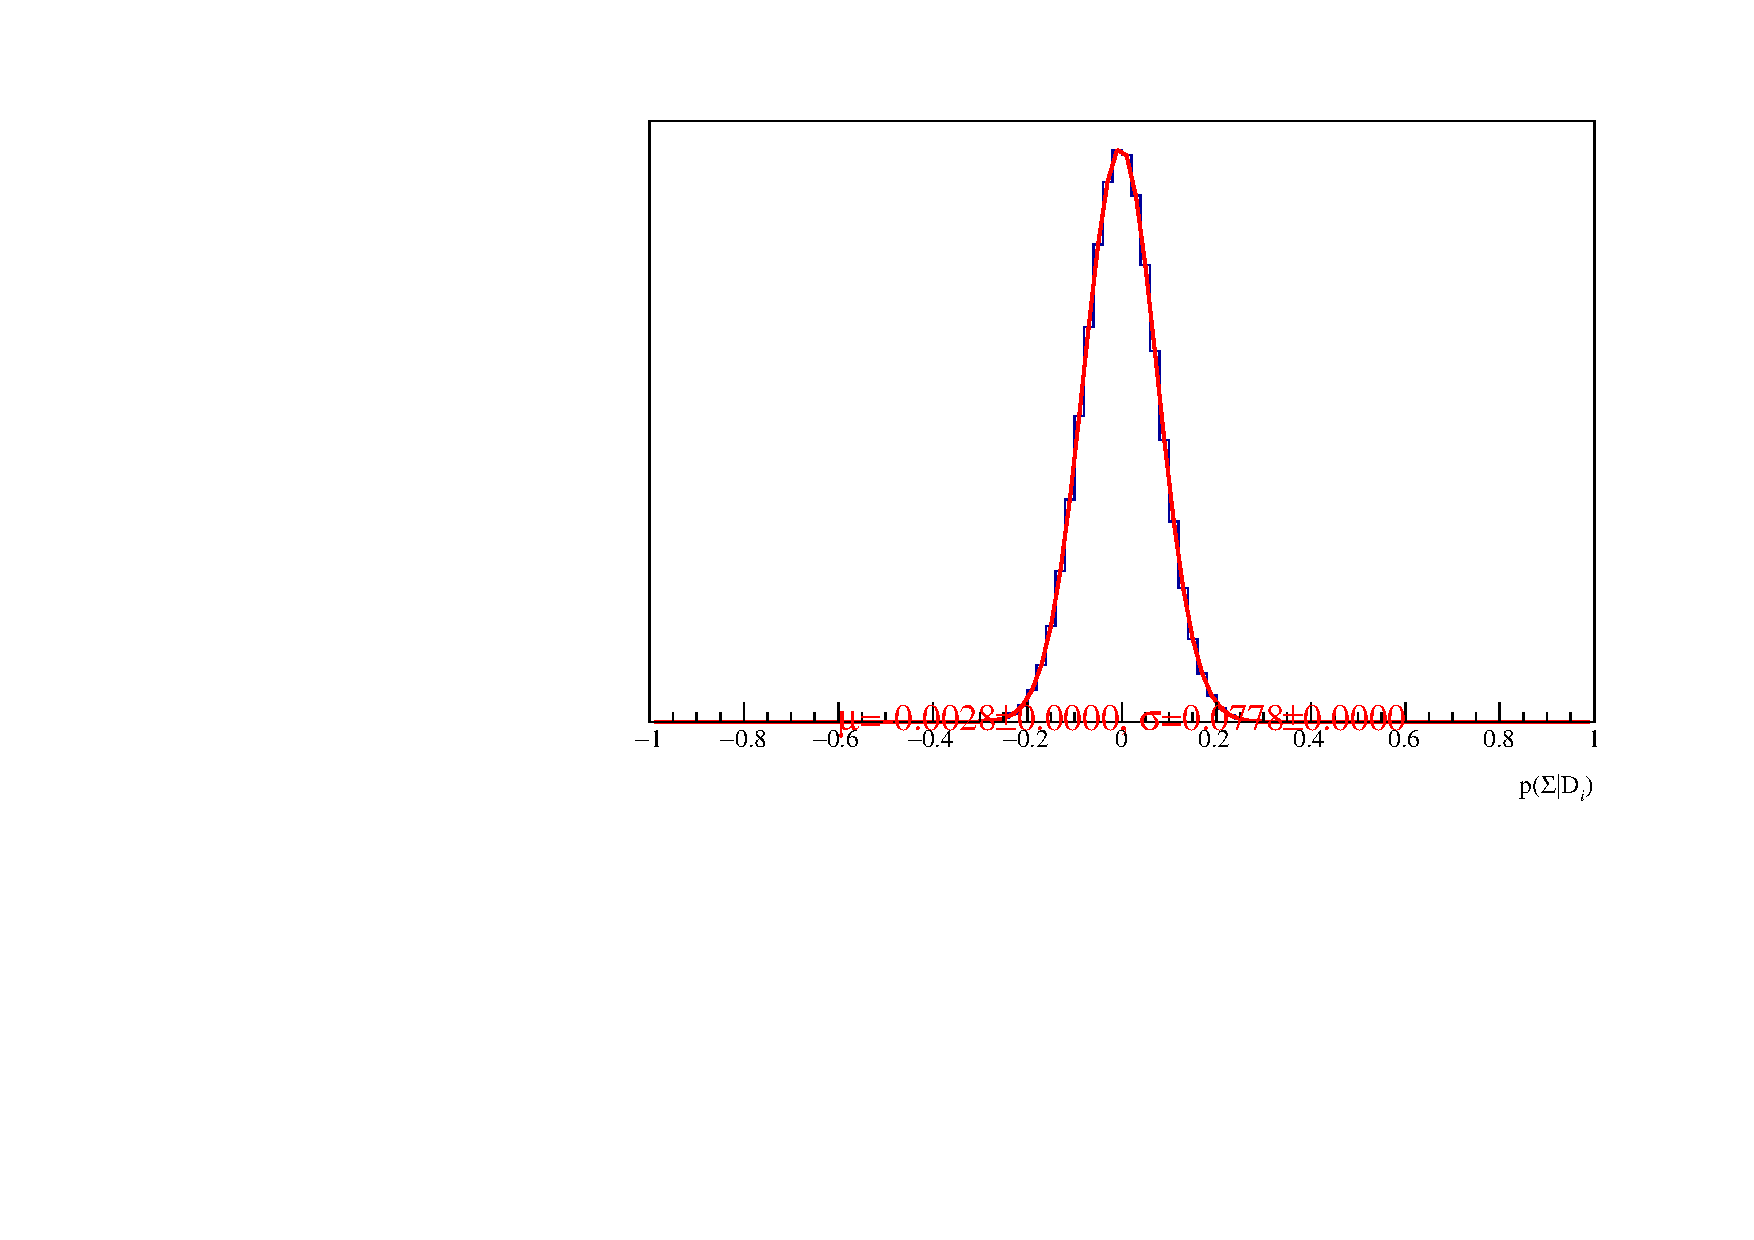
\includegraphics[width=.49\linewidth]{../../bayes/toyMC/plots/pi0_combined_post_add_raw.pdf}
		\end{figure}
		
	\end{frame}
		\begin{frame}{Fit results (event yield asymmetries with $\chi^2$ fit)}
		\begin{center}
			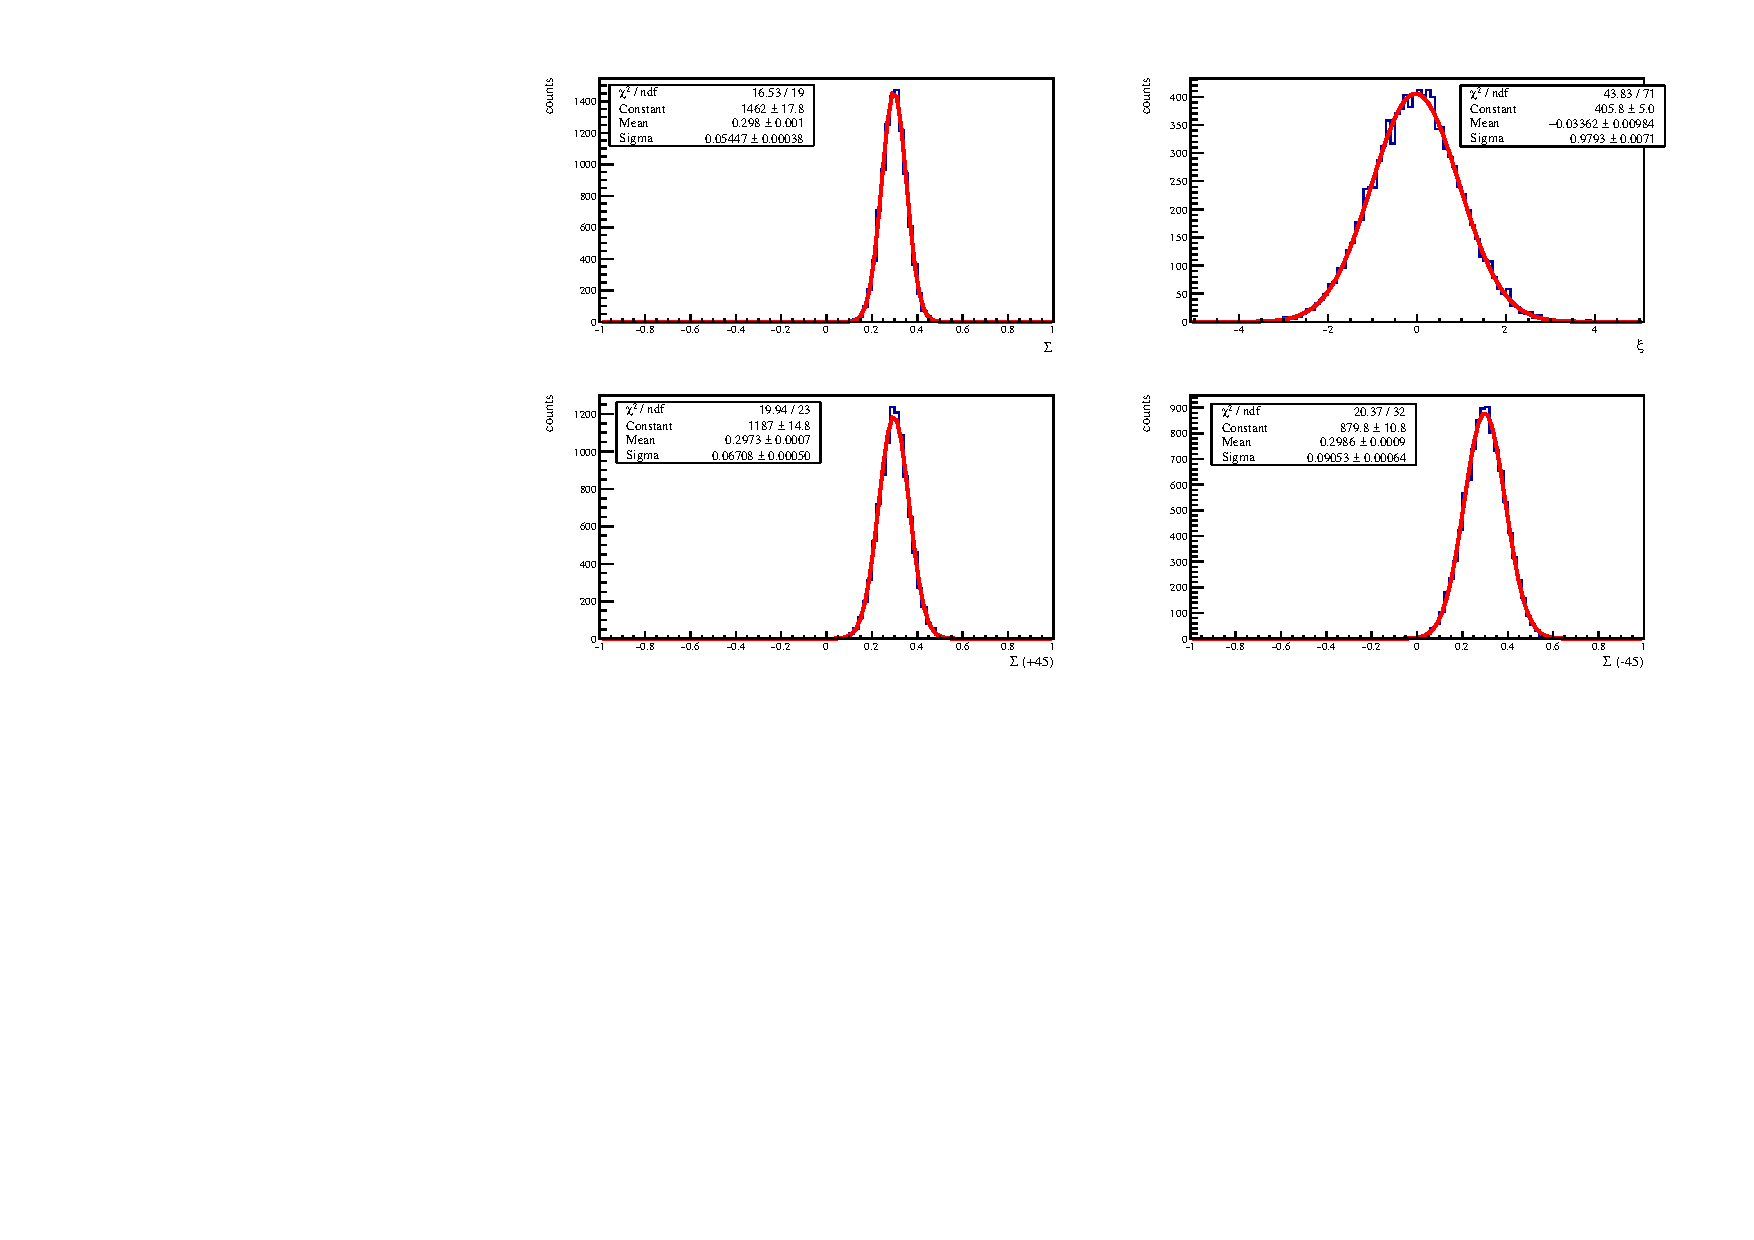
\includegraphics[width=.9\linewidth]{../../bayes/toyMC/plots/pi0_chi2.pdf}
		\end{center}
		
		
		Event yield method okayish, but binning and statistics affect the fit siginificantly!	
		
	\end{frame}
\begin{frame}{Fit results (Event-based fit)}
		\begin{itemize}[label=$\blacktriangleright$]
	\item 300 toy bins (fit takes very long)
	\item $p_\gamma^\parallel=0.25,p_\gamma^\bot=0.3$, $\Sigma=0.3$, sideband events and weights similar to data, Eff. func: $f(\phi)=\frac{1}{10.5}(9.3+0.28\cos\phi+0.24\sin3\phi)$
	\item $n_\text{events}^\parallel\sim\text{Pois}(800)$, $n_\text{events}^\bot\sim\text{Pois}(1000)$ 
	\item either build "normalized residuals" $\Xi$ or "independent likelihood pool" $P(\Sigma|y_0\dots y_{300})\propto\frac{\prod_ip(\Sigma|y_i)}{\pi(\Sigma)^{300-1}}$
\end{itemize}
\end{frame}
\begin{frame}{Fit results (Event-based fit)}
	\centering
	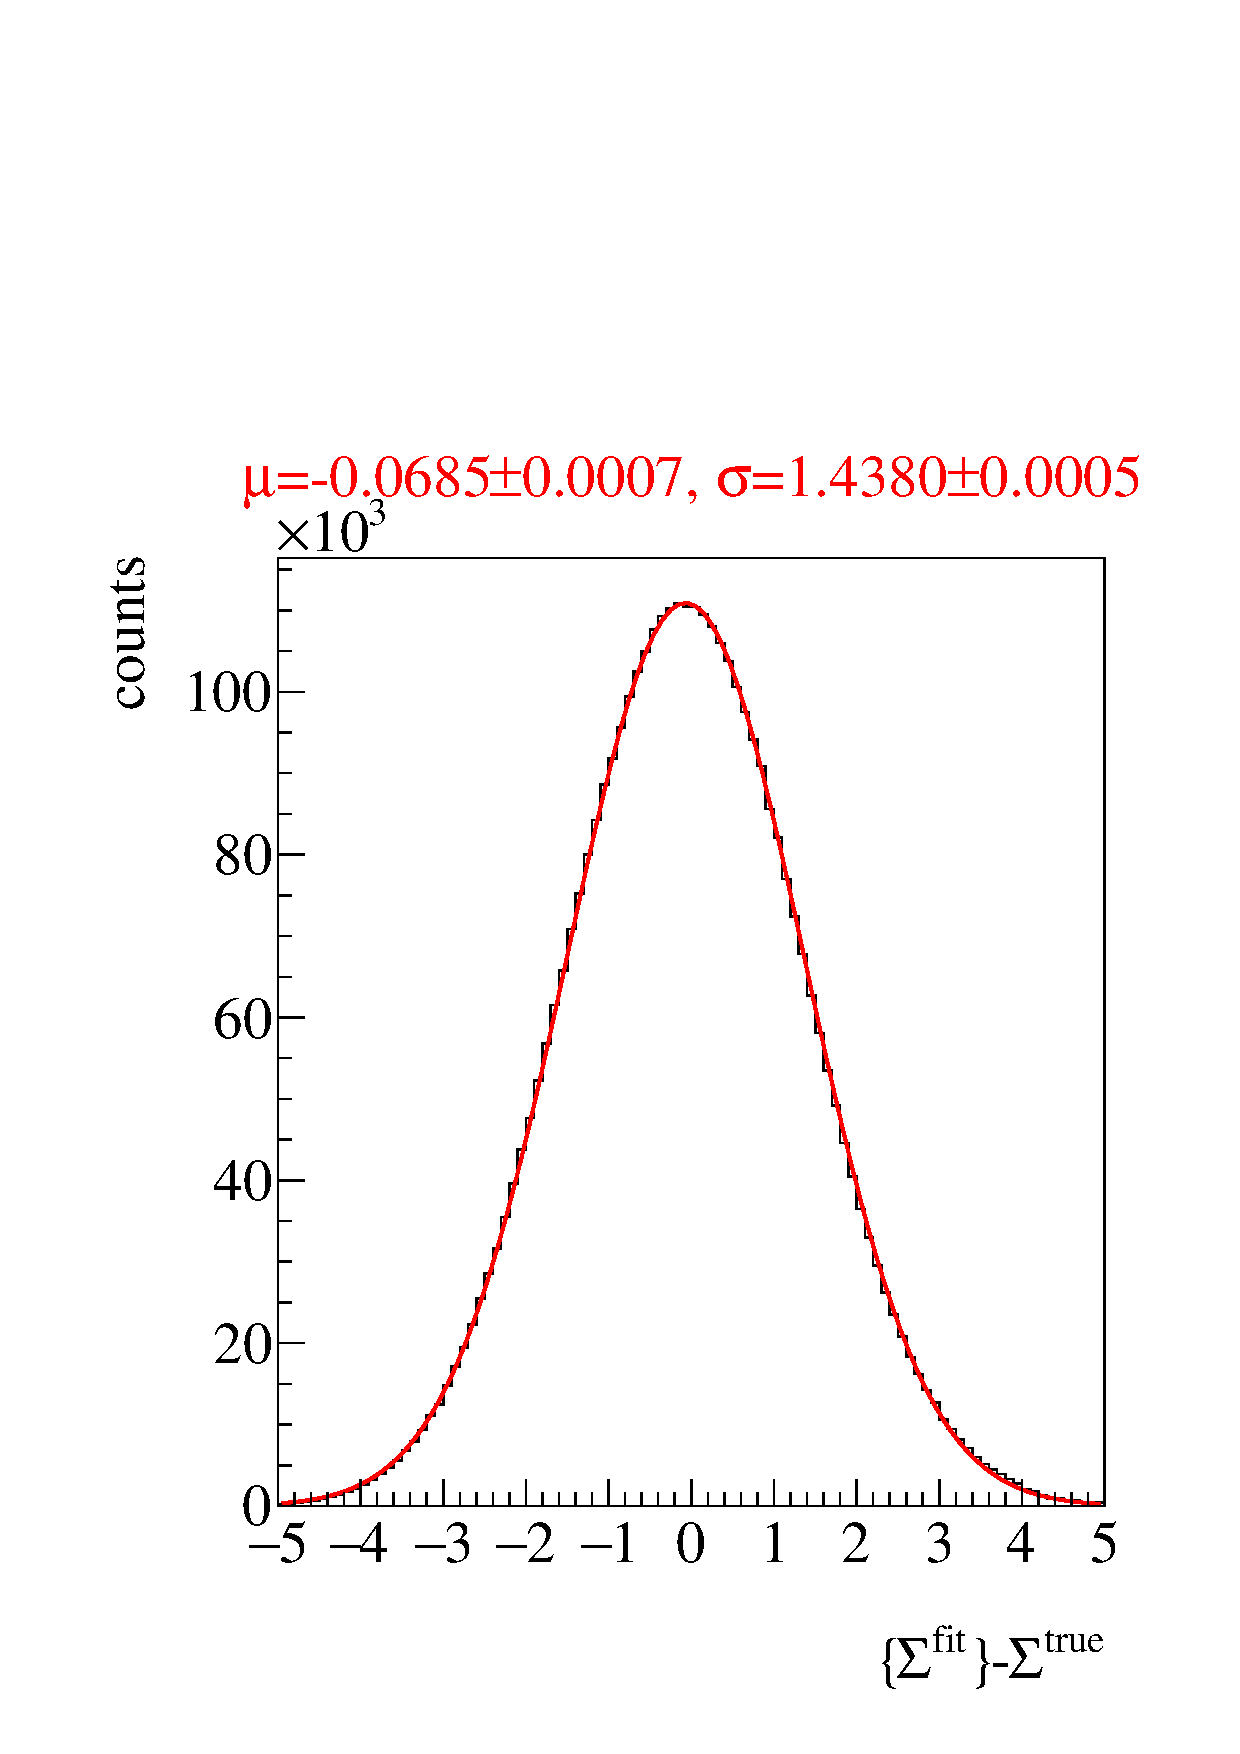
\includegraphics[width=.49\linewidth]{../../bayes/event_based_fit/plots/combined_post_add.pdf}
	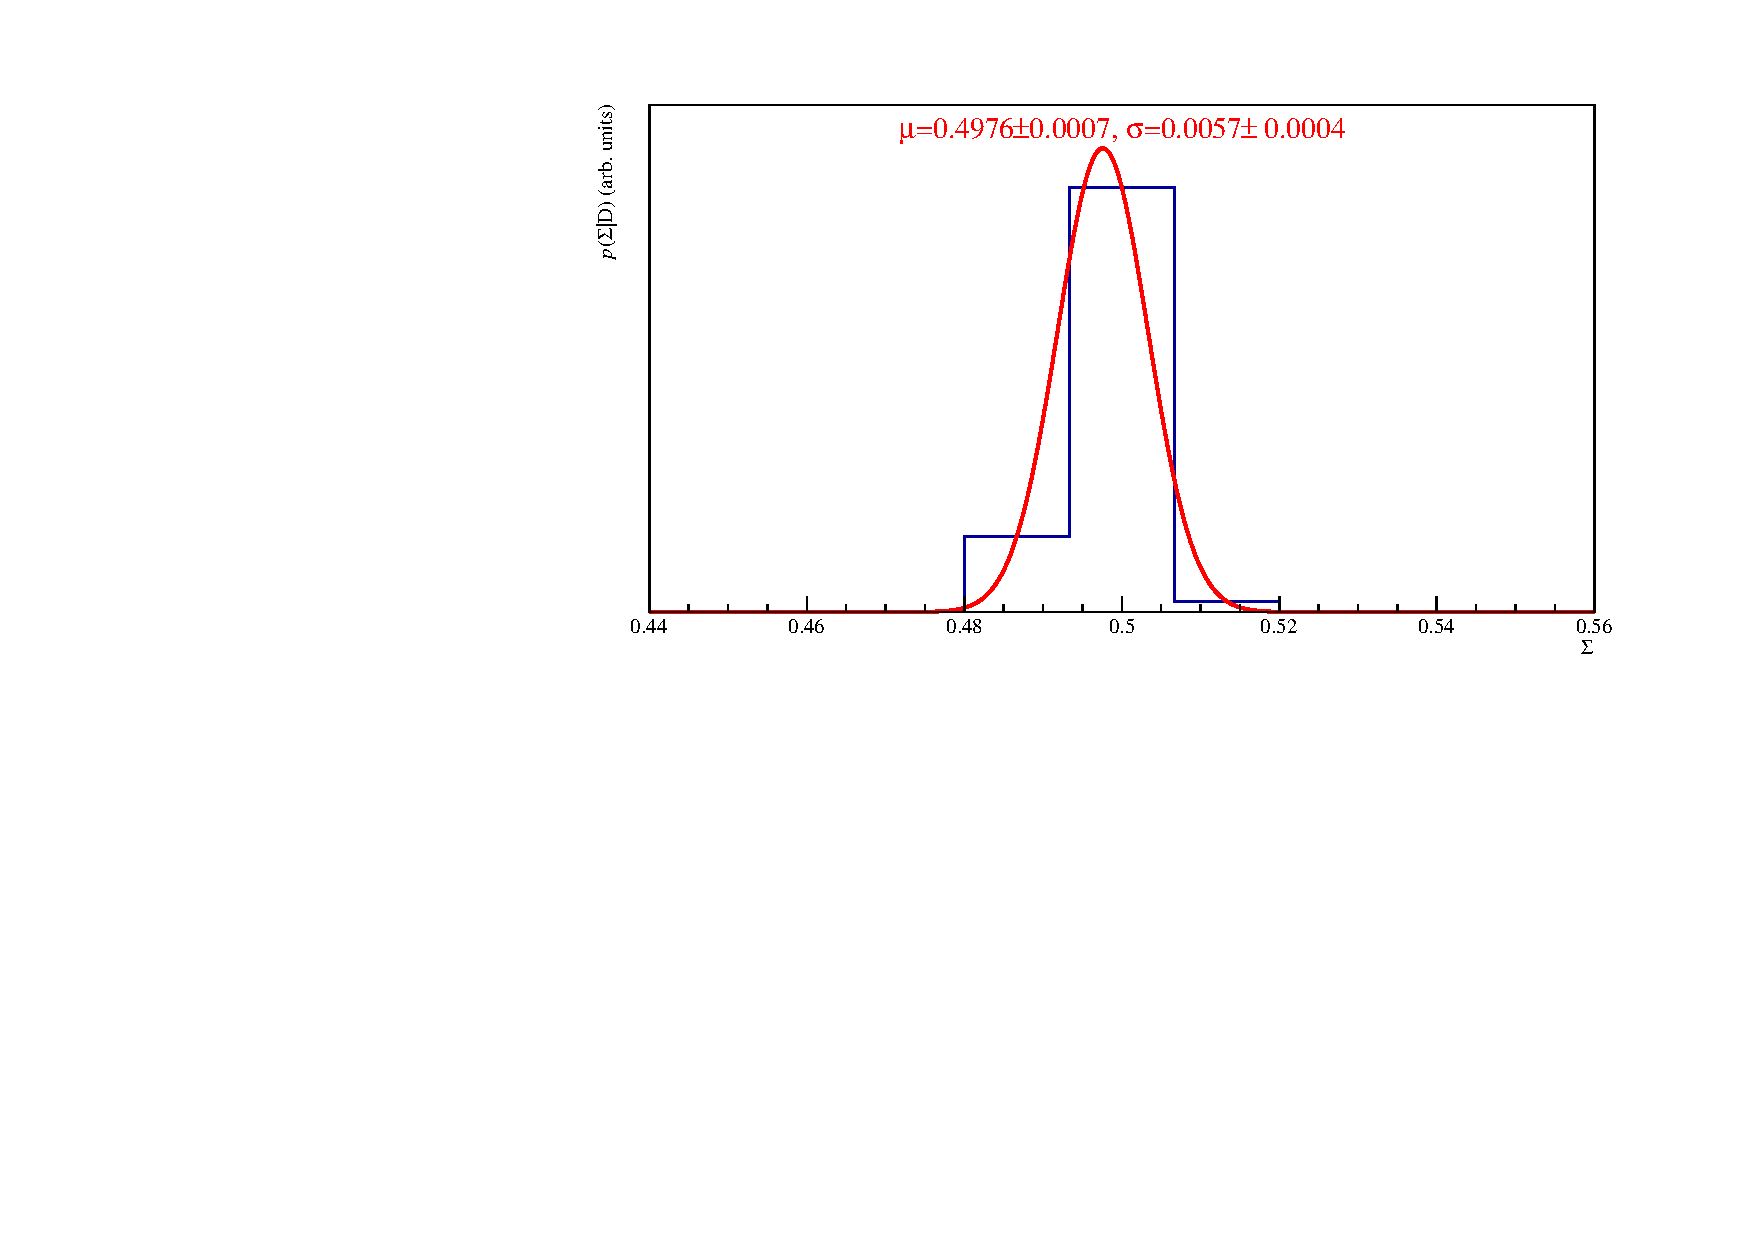
\includegraphics[width=.49\linewidth]{../../bayes/event_based_fit/plots/combined_post_mul.pdf}
	\end{frame}
\begin{frame}{Fit results (Event-based fit)}
		\centering
		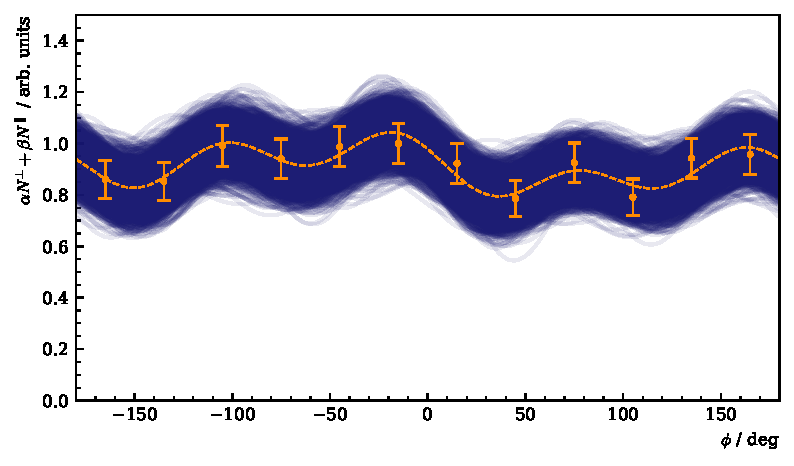
\includegraphics[width=.8\linewidth]{../../bayes/event_based_fit/plots/toyMC_eff_PPC.pdf}
\end{frame}
\begin{frame}{Fit results (Data), now "justified" :)}
	\centering
		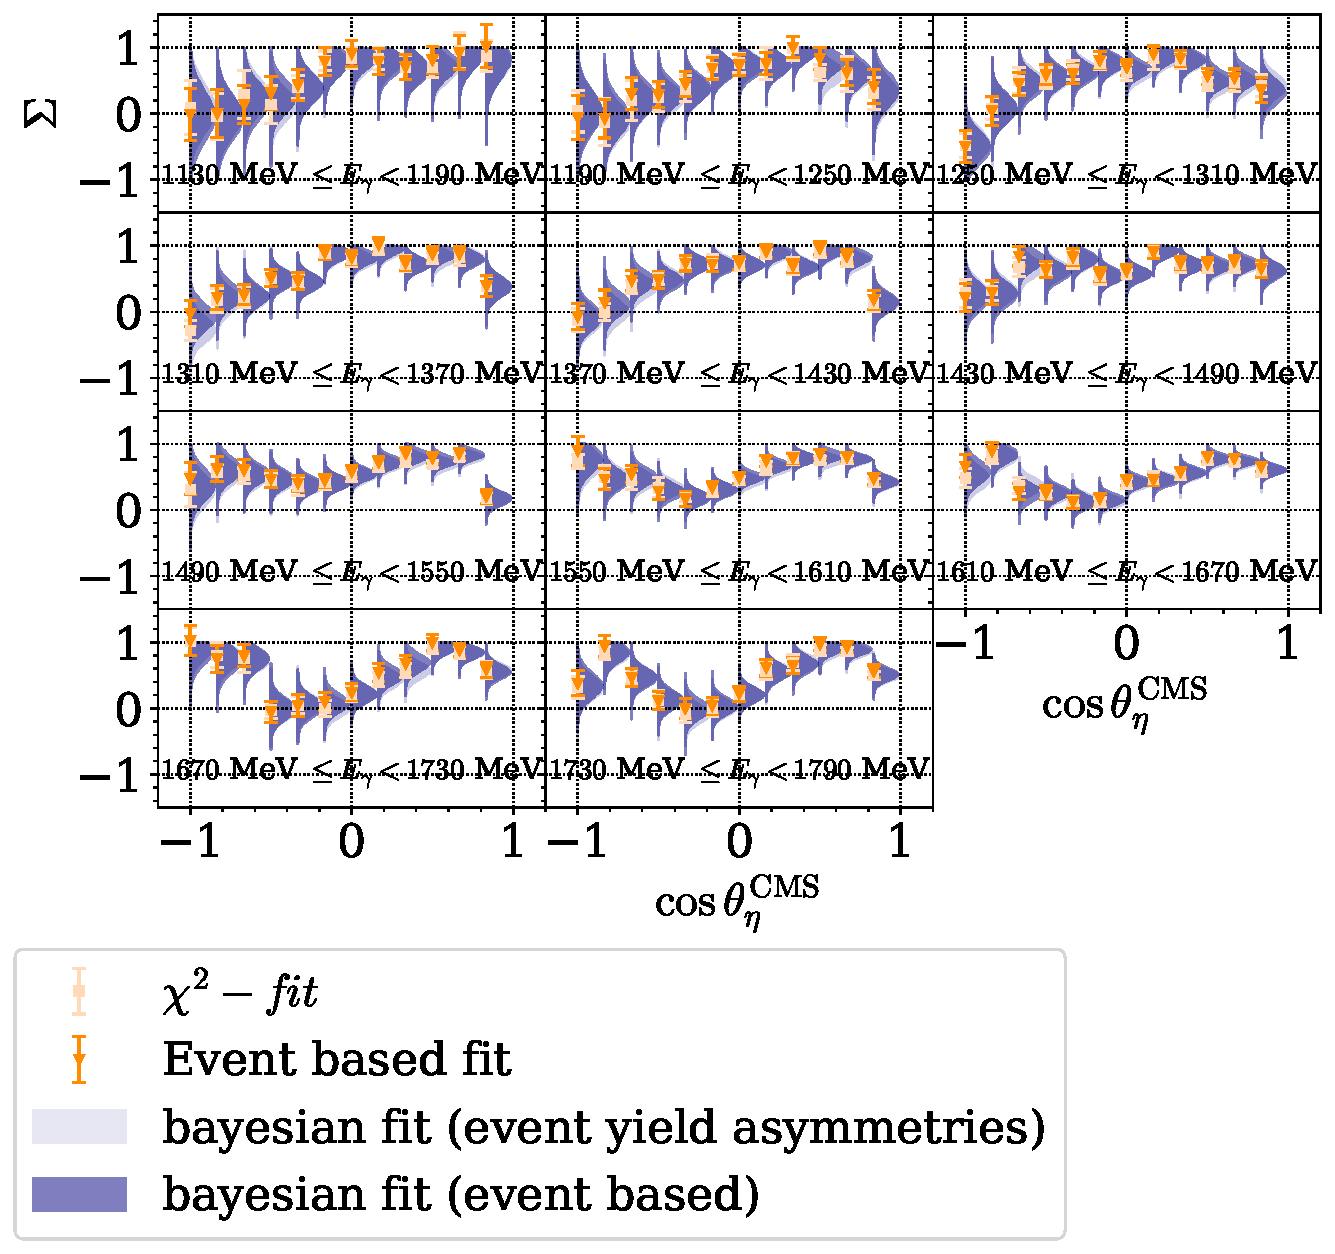
\includegraphics[width=.6\linewidth]{../../bayes/event_based_fit/plots/sigma_eta_alt.pdf}
\end{frame}
	
	
	
	
	
\end{document}
